\documentclass[9pt,twocolumn,twoside]{../../styles/osajnl}
\usepackage{fancyvrb}
\journal{i524} 

\title{Xen: A bare metal hypervisor}

\author[1]{Piyush Rai}


\affil[1]{School of Informatics and Computing, Bloomington, IN 47408, U.S.A.}

\affil[*]{Corresponding authors: piyurai@iu.edu}

\affil[+]{HID - S17-IO-3014}

\dates{\today}

\ociscodes{Baremetal hypervisor, Xen}

% replace this with your url in github/gitlab
\doi{\url{https://github.com/piyurai/sp17-i524/tree/master/paper1/S17-IO-3014/report.pdf}}


\begin{abstract}
\href{https://www.xenproject.org/}
{Xen} is an open-source baremetal hypervisor. This paper explores it's overview, architecture and contains a brief note on its alternatives.\newline
\end{abstract}

\setboolean{displaycopyright}{true}

\begin{document}

\maketitle

\section{Introduction}

To provide an isolated environment to different applications in terms of memory, process scheduling and disk access such that one process does not impact the other, used to be a major challenge for system administration \cite{xenvirtualization}. Also, different applications may have different OS requirements. Running an application within its own OS environment should protect it from other malicious applications because of the guranteed memory and disk allocation to each guest VM (virtual machine).

Xen is a baremetal hypervisor and the only one to be available as open-source \cite{www-xen-wiki}. It's based on microkernel design with the advantage of small memory footprint and has a limited guest interface. It’s responsibility is to manage CPU and memory, and to handle interrupts. Virtual machines are deployed in the guest domain called DomU which has no access privilege to hardware. A special virtual machine is deployed in the control domain called Domain 0. It contains hardware drivers and the toolstack to control the VMs and is the first VM to be deployed after the system comes up. The hypervisor is the first process to be started after bootloader.

\section{Architectural Overview and Use Cases}

Xen has a small memory footprint and provides limited interface to guest VMs. It runs at the highest CPU privilege level while the guests are deployed in DomU domain \cite{www-xen-wiki}. It's primary responsibility is to manage CPU, memory and interrupts and does not contains the drivers for I/O functions such as networking and storage. The main device driver for a system can be run inside of a virtual machine. It protects the rest of the system from events such as driver crashes as the VM containing the driver can be rebooted independently. The control stack is generally deployed on a Linux VM running in domain 0. It is the first VM to be deployed by the system and can access the hardware directly. It handles system's I/O functions and provides interface to control the system. It's responsible for creating and configuring VMs, allocating resources and monitoring them and terminating the VMs when they are no longer required. The control stack interface can also be driven through a cloud orchestration stack such as OpenStack. Figure \ref{fig:xen-arch} shows the architectural overview of Xen.

\begin{figure}[htbp]
	\centering
	\fbox{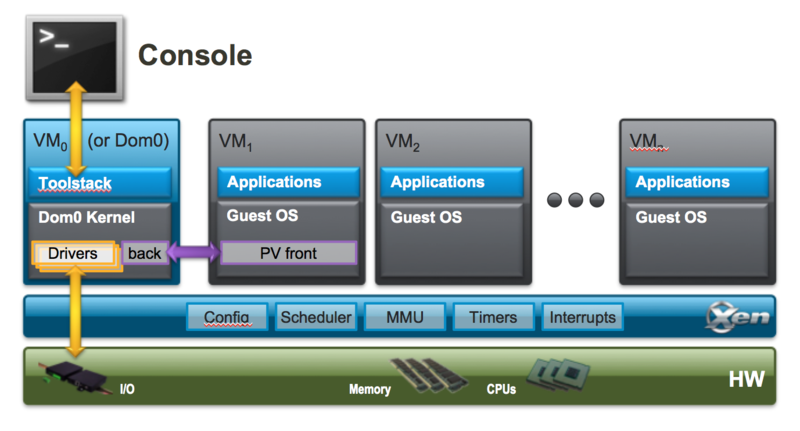
\includegraphics[width=\linewidth]{images/xen-arch.png}}
	\caption{Xen architecture overview \cite{www-xen-arch-diag}.}
	\label{fig:xen-arch}
\end{figure}

The guest virtual machines are deployed in domain DomU which has no privilege to access the hardware. The guest VMs can either be deployed in Para virtualization (PV) mode or Hardware-assisted virtualization mode (HVM). It's also possible to use PV drivers inside of a HVM mode to improve its performance. The two types of modes can be deployed simultaneously  on a single hypervisor. PV guests work without virtualization support from the hardware, and require PV-enabled kernel and drivers. The application binaries do not need any modification and run as in their native environments.  HVM uses virtualization support available on the host CPU such as Intel VT or AMD-V hardware extensions. QEMU is used to emulate the remaining PC hardware. No changes to kernel are required for fully virtualized guests. HVM guests can also use PVHVM drivers i.e. special  paravirtual device drivers optimized for HVM environments to boost up the performance. PVH is a recently developed new virtualization mode where  PV guests uses PV drivers for boot and I/O and hardware extensions otherwise. It is expected to simplify the Xen architecture and is the recommended virtualization mode to be used with newer Xen releases \cite{www-xen-pvh}. 

\section{Resources}

The Xen Project wiki page presents an overview of the software architecture and host the links to dcocumentation and release notes for the different releases, e.g. the list of feature for release 4.8 can be found at \cite{www-xen-4.8-release-note}. David Chisnall has also witten a \href{http://www.informit.com/store/definitive-guide-to-the-xen-hypervisor-9780133582499} {book} explaining the hypervisor internals and it's important features along with their interfaces. 

\section{Alternatives}

\cite{www-kvm-evolution} talks about the limitations during the early days of Xen development like modification to the guest kernels and limited Linux support. The article here \cite{www-kvm-rise} states about later years into the development of Xen, when it remained based on the older version of Linux kernel as the developers waited for more recent kernels with support for modern hardware. This allowed KVM to overtake as preferred choice for virtualization. KVM overcame the problems faced by Xen by using the virtualization support in the newly available hardware and reusing the components from the Linux kernel. This gave it the advantage of automatically benefiting from the developments in the mainline kernel. Its incorporation into the Linux version 2.6.20 and contribution from companies like AMD and Intel increased KVM's adaptability among the Linux distributors.

KVM requires hardware assisted virualization with new releases containing paravirtualization support for certain devices \cite{www-kvm-wiki}.Xen was originally developed to overcome the problem of limited support for hardware assisted virtualization \cite{www-xen-pvh} by using Paravirtualization. Xen is a layer between the kernel and hardware whereas KVM turns the kernel itself into the hypervisor. Xen has it's own memory and power management system designed specifically for VMs where as KVM needs to have support for processes as well.

In his blog \cite{www-tech-comparison} Bredan Gregg has listed the observations made during comparisons of different virtualization technologies at Joyent using DTrace. It analyzed the stack trace for different system functionalities such as network and I/O calls stack trace along with the relevant overhead for Zones, Xen and KVM. It mentioned about Zones, with Linux Containers being its equivalent, to be the preferred choice for virualization for them as it has the lowest overhead for not having to run an entire OS for each application. They stopped using Xen in favor of KVM for provisioning fully virualized guest machines.

\section{Current Status and The Future}

Xen is actively maintained by Linux Foundation under the trademark “XEN Project”. Some of the features included in the latest releases include “Reboot-free Live Patching” (to enable application of security patches without rebooting the system) and KCONFIG support (compilation support to create a lighter version for requirements such as embedded systems) \cite{www-xen-4.7-feature-list}. The overheads in terms of passing data across several layers is being minimized by use of shared memory transports and buffers \cite{www-tech-comparison}. Xen Project also strives to minimize the foorptint of the change to Linux kernel. The codebase contains less than 150,000 lines of code \cite{www-xen-wiki}. Xen Project hosts a \href{https://xenproject.org/directory/directory.html} {lisiting} of vendors that uses Xen Project software to allow them to advertise their software and services. Xen is used by more than 10 million users \cite{www-hypervisor-17} . Some of the major cloud hosting service providers using Xen include Amazon and Rackspace. Hypervisors are predictedd to become a core aspect of cloud based solutions. Containers are grwoing in popularity and there's an increasing interest in combination of isolation aspects of hypervisor and container runtime environments \cite{www-hypervisor-containers}.  Bellani has witten a comprehensive blog [11] about the ongoing work within Xen community towards the development of hypervisor-based containers.


% Bibliography

\bibliography{references}
 

\end{document}
